% ----------------------------------------------------------------------------------------------
% TEMPLATE PARA TRABALHO DE CONCLUSÃO DE CURSO
% Universidade Federal do Pará
% Modelo da Faculdade de Engenharia Elétrica
% Idealizado por Sérgio Custódio e Kelvin Pinheiro
% Baseado no projeto: http://tcc.tsi.gp.utfpr.edu.br/paginas/modelos-latex-da-utfpr
% Baseado na modificação de :       Diego Marczal e 
% 	          						Michael Vornes 
% ----------------------------------------------------------------------------------------------
% CARREGA CLASSE PERSONALIZADA DA FEEM/UFPA-----------------------------------------------------
\documentclass[%twoside,                   % Impressão em frente e verso
oneside,                                   % Impressão apenas frente
]{ufpa-fem-abntex2}


%INCLUI ARQUIVOS DO TRABALHO DE CONCLUSÃO DE CURSO (PRÉ-TEXTUAIS, TEXTUAIS, PÓS-TEXTUAIS)----------------------------------------------------------------------------------
%%%%%

% INSERE CAPA E FOLHA DE ROSTO
% CAPA-------------------------------------------------------------------------------------

% ORIENTAÇÕES GERAIS-------------------------------------------------------------------------------------
% Caso algum dos campos não se aplique ao seu trabalho, como por exemplo,
% se não houve coorientador, apenas deixe vazio.
% Exemplos: 
% \coorientador{}
% \departamento{}

% DADOS DO TRABALHO------------------------------------------------------------------------
\titulo{\textbf{TÍTULO DO TRABALHO}}
\subtitulo{subtítulo (se houver)} %Se não hover subtítulo, deixar em branco.
\titleabstract{Title in English}
\autor{Oséias Dias de Farias}
\autorcitacao{ÚLTIMO NOME, Nome} % Sobrenome em maiúsculo
\local{TUCURUÍ/PA}
\data{2023}

% NATUREZA DO TRABALHO-----------------------------------------------------------------------------------
\projeto{Trabalho de Conclusão de Curso}

% TÍTULO ACADÊMICO-------------------------------------------------------------------------
\tituloAcademico{Bacharel}

% ÁREA DE CONCENTRAÇÃO E LINHA DE PESQUISA-----------------------------------------------------------------------------------
% Se a natureza for Trabalho de Conclusão de Curso, deixe ambos os campos vazios
% Se for programa de Pós-graduação, indique a área de concentração e a linha de pesquisa
\areaconcentracao{}
\linhapesquisa{}

% DADOS DA INSTITUIÇÃO---------------------------------------------------------------------
% Se a natureza for Trabalho de Conclusão de Curso, coloque o nome do curso de graduação em "programa"
% Formato para o logo da Instituição: \logoinstituicao{<escala>}{<caminho/nome do arquivo>}
\instituicao{Universidade Federal do Pará}
\departamento{Instituto de Tecnologia}
\programa{Faculdade de Engenharia Elétrica}
\logoinstituicao{2cm}{figuras/naomexafig/logoufpa.png} %

% DADOS DOS ORIENTADORES-------------------------------------------------------------------
\orientador{Prof. Esp. XXXX XXXXX XXXXXXX}
%\orientador[Orientadora:]{Nome da orientadora}
\instOrientador{Universidade Federal do Pará}

%\coorientador{Nome do coorientador}
%\coorientador[Coorientadora:]{Nome da coorientadora}
%\instCoorientador{Instituição do coorientador}

% FOLHA DE ROSTO----------------------------------------------------------------------------

% Este arquivo não precisa ser alterado

%% TRABALHO DE CONCLUSÃO DE CURSO
\preambulo{{\imprimirprojeto}, apresentado como requisito parcial para a obtenção de grau de {\imprimirtituloAcademico} em Engenharia Elétrica, pela {\imprimirinstituicao}.}

% ---
% Inserir folha de aprovação
% ---
% Isto é um exemplo de Folha de aprovação, elemento obrigatório da NBR
% 14724/2011 (seção 4.2.1.3). Você pode utilizar este modelo até a aprovação do trabalho. Após isso, substitua todo o conteúdo deste arquivo por uma imagem da página assinada pela banca com o comando abaixo:
%
% \includepdf{folhadeaprovacao_final.pdf}
%


\dataaprovacao{08/03/2019}
\conceito{} %Antes da defesa, não adicionar valor ao compo. Após a defesa, pode-se adicionar Regular, Bom ou Excelente e solicitar as assinaturas da banca examinadora.
 
\nomePrimeiromembro{Prof. Esp. Sérgio de Souza Custódio Filho}
\instPrimeiromembro{FEM/ITEC/UFPA}
 
\nomeSegundomembro{Prof. Me. Fábio Antônio do Nascimento Setúbal}
\instSegundomembro{FEM/ITEC/UFPA}

%Ocultar ou não dependendo do numero de professores na banca. Ver arquivo de configuracao \assinatura{\imprimirnomeTerceiromembro  \\ Membro - \imprimirinstTerceiromembro}  nas configuracoes ufpa-fem-abntex2.cls.

%\nomeTerceiromembro{Eng. Beltrano Cunha} 
%\instTerceiromembro{Externo (PETROBRAS)}

%ª
 


\begin{document}
	
	\pretextual
	\imprimircapa                                  
	\imprimirfolhaderosto{}                           
	\imprimirfolhadeaprovacao{}                       
	% DEDICATÓRIA------------------------------------------------------------------

\renewcommand{\dedicatorianame}{DEDICATÓRIA}

\begin{dedicatoria}

Dedico aos meus pais e a toda a minha família.

\end{dedicatoria}
          			
	% -------------------------------------------------------------------------------------------------
% Inserir os agradecimentos:
% -------------------------------------------------------------------------------------------------

\begin{agradecimentos}

À minha mãe e meu pai que dedicaram suas vidas por esse propósito, Aos professores do curso pela dedicação em simplificar o complexo, em especial aos professores da área de sistema de controle;\\
Finalmente, ao meu orientador Prof. Dr. Raphael Teixeira pela sua orientação e paciência.

\end{agradecimentos}
% ---

	% EPÍGRAFE---------------------------------------------------------------------

\renewcommand{\epigraphname}{EPÍGRAFE}

\begin{epigrafe}

\textit{``A matemática é o alfabeto no qual Deus escreveu o universo.'' (Galileu Galilei)}

\end{epigrafe}

% OBSERVAÇÕES------------------------------------------------------------------
% Altere o texto para inserir a epígrafe do seu trabalho


	% RESUMO--------------------------------------------------------------------------------

\begin{resumo}[RESUMO]
\begin{SingleSpacing}

Escreva seu resumo aqui!!!\\

\textbf{Palavras-chave}: Palavra-chave 1. Palavra-chave 2. Palavra-chave 3. Palavra-chave 4.

\end{SingleSpacing}
\end{resumo}

% OBSERVAÇÕES---------------------------------------------------------------------------
% Altere o texto inserindo o Resumo do seu trabalho.
% Escolha de 3 a 5 palavras ou termos que descrevam bem o seu trabalho .
% As palavras-chave são separadas por pontos. Apenas a primeira letra é maiúscula.

 								% Resumo em Português
	% ABSTRACT--------------------------------------------
\begin{resumo}[\textbf{ABSTRACT}]

\textit{This work presents a comprehensive virtual laboratory for the study of control systems, which combines the integration of a physical prototype, 3D simulator and an interactive graphical interface. The motivation for this project lies in the intrinsic complexity associated with understanding control systems, which often presents challenges, especially for students who need to overcome the barrier of abstracting physical systems in terms of mathematical equations. To develop the project, an Aeropendulum prototype was implemented, complete with a set of software that allows the user to interact with the physical system, enabling the user to make changes to the system's parameters in real time. In addition, a digital twin was developed to mirror the dynamics of the Aeropendulum prototype using a 3D simulator. Finally, tests were carried out to validate the laboratory, including: application of system identification using discrete transfer function and least squares and closed loop testing with a PID controller. The project has been hosted on GitHub in order to disseminate knowledge and allow enthusiasts, students and researchers to have access to the complete project, The combination of prototypes, simulators, graphical interface and integration of various Electrical Engineering disciplines creates an engaging and effective learning environment for the study of control systems. This approach reduces students' initial resistance and promotes a deeper understanding of the concepts and applications in this area. Through practice, students can see the relevance of mathematical abstractions in solving real problems, preparing them to deal with complex and challenging control systems.}\\

\textbf{Keywords}: \textit{Aeropendulum, system identification, prototype, simulator, digital twin}.
\end{resumo}
 							% Resumo em Inglês
	\include{pre-textuais/naomexapretext/lista-figuras}
	%\include{pre-textuais/naomexapretext/lista-quadros}
	\include{pre-textuais/naomexapretext/lista-tabelas} 		% Lista de Tabelas
	% LISTA DE ABREVIATURAS E SIGLAS----------------------------------------------------------

\begin{siglas}
    \item[BET] Teoria do Elemento de Pá (\textit{Blade Element Theory})
    \item[THEV] Turbina Hidrocinética de Eixo Vertical
    \item[THEH] Turbina Hidrocinética de Eixo Horizontal ...
\end{siglas}

% OBSERVAÇÕES-----------------------------------------------------------------------------
% Altere a lista acima para definir os acrônimos e siglas utilizados neste trabalho
          		
	\include{pre-textuais/lista-simbolos}
	%\include{pre-textuais/naomexapretext/lista-algoritmos}
	\include{pre-textuais/sumario} 								% Sumário              			   
	%Verificar folha de Aprovação e Catalogação Bibliográfica
	
	\textual
	% INSERE ELEMENTOS TEXTUAIS
	% INTRODUÇÃO-------------------------------------------------------------------

\chapter{INTRODUÇÃO}
\label{chap:introducao}

Alguns programas podem ser utilizados para auxílio da escrita do TCC entre eles o \textit{MathType} (com relação a equações), \textit{Inkscape} (com relação a imagens). \\ %enter

\textbf{PRIMEIRAS ORIENTAÇÕES}\\ %\textbf - negrito

1) O comando ``$\backslash$autoref\{label\}'' auto referencia o respectivo ``\textit{label}".

Exemplo 1: De acordo com o exposto no \autoref{chap:introducao}... Pode-se verificar na \autoref{fig:consumomundialporfonte-fig1}...\\

2) O comando ``$\backslash$citeonline\{bibid\}'' é utilizado para citações diretas. Ele cita o respectivo ``\textit{bibid}".\\

Exemplo 2:  Conforme \citeonline{AMARANTEMESQUITA20141261} cita em seu artigo, turbinas hidrocinéticas atualmente têm... \citeonline{VAZ2018509} também ressalta que turbinas de eixo horizontal possuem maiores...\\

\citeonline{vallverdu2014}  --->  Vallverdú (2014) --- DIRETA

\cite{vallverdu2014}   --->  (VALLVERDÚ, 2014) --- INDIRETA\\

O comando ``$\backslash$cite\{bibid\}'' é utilizado para citações indiretas. Ele cita o respectivo ``\textit{bibid}".\\

Exemplo 3: A máxima eficiência que uma turbina hidrocinética ideal pode alcançar é dada pelo Limite de Betz-Joukowski que corresponde a 59,3\%, o equivalente a um $C_P$ de 0,593 \cite{vallverdu2014, SHINOMIYA2015d}.\\ %Ao colocar a virgula, pode-se adicionar mais de um autor à citação.

3) Um ponto final é representado por um espaço entre os parágrafos.

Exemplo 1.
Exemplo 2.

Exemplo 3.

Exemplo 4.\\

4) Figuras

Figuras com extensão .jpg, .pdf, .eps, .ps, .png

As figuras devem ser adicionadas a pasta ``$\backslash$figuras'' no diretório deste template.

%[!htb] - são as opções onde o LaTeX escolhe a melhor posição para inserir a figura na página, aqui (here), topo (top) ou embaixo (bottom), respectivamente. Se você colocar apenas um deles, por exemplo [!h], a figura ficará exatamente onde você inseriu.

%Modelo de inclusão de figura. É só copiar, tomar como modelo e modificar.
\begin{figure}[H]
	\centering
	\caption{Consumo mundial de energia por fonte de energia em quatrilhões de BTU.}
	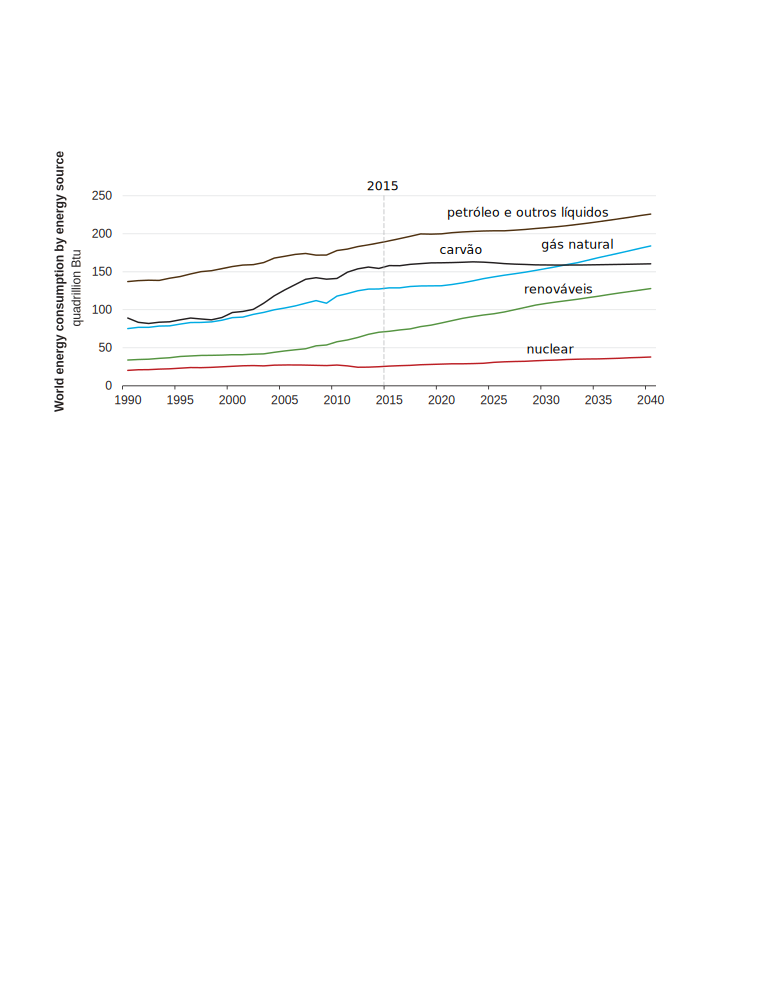
\includegraphics[width=1.0\textwidth]{figuras/consumodeenergiamundialporfonte.pdf}
	\fonte{\citeonline{harris2006essential}.}
	\label{fig:consumomundialporfonte-fig1}
\end{figure}

5) Referências

As referências devem ser adicionadas no arquivo ``base-referencias.bib'' no diretório deste template. 

Modelos podem ser editados na página ``https://truben.no/latex/bibtex/''. A partir do DOI pode-se encontrar o arquivo \textit{.bib} em ``https://www.doi2bib.org/''. No Google Acadêmico também se encontram bastantes referências no formato \textit{.bib}.

Tome cuidado com autores com nomes que termiam em Júnior, Filho, Neto e etc. Forma correta: ``Fulano Deltrano Siclano\{ \}Neto''.

As referências não reconhecem legal os pacotes de acentos. Então deve-se utilizar comandos de acentos. ``http://latexbr.blogspot.com/2011/02/acentos-e-caracteres-especiais.html''.

*Ao ser executado pela primeira vez, possa ser que você precise está conectado a internet para o programa instalar os \textit{packages} necessários para compilar o arquivo PDF.

Utilize esse \textit{template} sempre verificando as normas da Biblioteca Central da UFPA segundo o Guia para Elaboração de Trabalhos Acadêmicos disponível em http://bc.ufpa.br/ além das normas da ABNT.

Outras orientações podem ser encontradas na internet.\\

Boa escrita!

\section{Objetivos}
\label{sec:objetivos}

\subsection{Objetivo geral}
\label{subsec:objetivogeral}

Escreva seu objetivo geral aqui.

\subsection{Objetivos específicos}
\label{subsec:objetivosespecificos}

\begin{itemize}
\item Escreva seu objetivo específico 1 aqui;
\item Escreva seu objetivo específico 2 aqui;
\item ...;
\end{itemize}

\section{Estrutura do trabalho}
\label{sec:estrututaTrabalho}

Este trabalho está dividido em cinco seções, referências, anexos e apêndices.

Na seção 1 é apresentado o contexto no qual o trabalho está inserido, a justificativa e os objetivos almejados...

A revisão bibliográfica sobre as temáticas relacionadas com essa pesquisa é apresentada na seção 2...

A seção 3 mostra conceitos teóricos relacionados às ferramentas utilizadas no estudo tal como...

Na seção 4, os resultados são apresentados juntamente com suas devidas discussões, verificando...

Finalizando, a seção 5 faz as devidas conclusões e apresenta sugestões para trabalhos futuros.

	% REVISÃO DE LITERATURA--------------------------------------------------------

\chapter{REVISÃO BIBLIOGRÁFICA}
\label{chap:fundamentacaoTeorica}

\section{Turbinas hidrocinéticas}

A potencia gerada por uma turbina pode ser expressa pela \autoref{eq:Power}.

\begin{equation}
P = \frac{1}{2}A\rho {V^3}{C_P}
\label{eq:Power}
\end{equation}

Sendo $A$ a área do rotor da turbina ($m^2$), $\rho$ a massa específica do fluido ($kg/{m}^3$), $V$ é a velocidade de corrente ($m/s$) e $C_P$ o coeficiente de potência (adimensional). O coeficiente de potência de uma turbina hidrocinética indica a quantidade de energia mecânica extraída a partir da energia disponível no fluido. A máxima eficiência que uma turbina hidrocinética ideal pode alcançar é dada pelo Limite de Betz-Joukowski que corresponde a 59,3\%, o equivalente a um $C_P$ de 0,593 \cite{vallverdu2014, SHINOMIYA2015d}.

\subsection{Princípios de funcionamento, classificação e principais componentes}

A \autoref{fig:Behrouzi2014-2} apresenta algumas configurações possíveis.

\begin{figure}
	\centering
	\begin{subfigure}{0.31\textwidth}
		\centering
		\includegraphics[scale=0.9]{figuras/VermaakVa.jpg}
		\caption{Eixo no plano.}
		\label{subfig:Inplane}
	\end{subfigure}
	\begin{subfigure}{0.31\textwidth}
		\centering
		\includegraphics[scale=0.9]{figuras/VermaakVf.jpg}
		\caption{Savonius.}
		\label{subfig:Savonius}
	\end{subfigure}
	\begin{subfigure}{0.31\textwidth}
		\centering
		\includegraphics[scale=0.9]{figuras/VermaakVd.jpg}
		\caption{Darrieus.}
		\label{subfig:Darrieus}
	\end{subfigure}
	\begin{subfigure}{0.31\textwidth}
		\centering
		\includegraphics[scale=0.9]{figuras/VermaakVc.jpg}
		\caption{Darrieus - H.}
		\label{subfig:DarrieusH}
	\end{subfigure}	
	\begin{subfigure}{0.31\textwidth}
		\centering
		\includegraphics[scale=0.9]{figuras/VermaakVb.jpg}
		\caption{Darrieus gaiola de esquilo.}
		\label{subfig:SquirrelcageDarrieus}
	\end{subfigure}
	\begin{subfigure}{0.31\textwidth}
		\centering
		\includegraphics[scale=0.9]{figuras/VermaakVe.jpg}
		\caption{Gorlov.}
		\label{subfig:Gorlov}
	\end{subfigure}	
	\caption{Turbinas hidrocinéticas de eixo vertical.}
	\fonte{\citeonline{harris2006essential}.}
	\label{fig:Behrouzi2014-2}
\end{figure}

\subsection{Modelos de predição de performance hidrodinâmica}

Uma revisão sobre modelos de predição de performance para turbinas eólicas de eixo vertical incluem os trabalhos de \citeonline{Brahimi1995}, \citeonline{paraschivoiu2002prediction}, \citeonline{paraschivoiu2002wind} e \citeonline{ISLAM20081087},  que serviram como ponto de partida para os modelos hidrodinâmicos \cite{Dai2011}. 

	% FUNDAMENTAÇÃO TEÓRICA--------------------------------------------------------

\chapter{FUNDAMENTAÇÃO TEÓRICA}
\label{chap:fundamentacao-teorica}

\section{Double-multiple streamtube model - DMST}
\label{sec:dmst}

Considerando a \autoref{fig:EsquemaVelocidade} que apresenta o comportamento das velocidades envolvidas em uma pá, a velocidade relativa ($u_r$) pode ser calculada pela \autoref{eq:Vrelativa}, o ângulo de trajetória ($\beta$) pela \autoref{eq:beta} e o ângulo de ataque ($\alpha$) pela \autoref{eq:alfa}, todos em função do ângulo azimute ($\theta$) da turbina.

\begin{figure}
	\centering
	\caption{Esquema do escoamento e forças na pá.}
	\includegraphics[width=0.7\textwidth]{figuras/EsquemaVelocidade.pdf}
	\fonte{ \citeonline{vallverdu2014}}
	\label{fig:EsquemaVelocidade}
\end{figure}

%Modelo de inclusão de equação. É só copiar, tomar como modelo e modificar.
\begin{equation}
{u_r} = \sqrt {{u^2} + {{(\dot \theta R)}^2} + 2u(\dot \theta R)\cos \theta }
\label{eq:Vrelativa}
\end{equation}

\begin{equation}
\beta  = \arctan \left( {\frac{{\dot \theta Rsen\theta }}{{u + \dot \theta R\cos \theta }}} \right)
\label{eq:beta}
\end{equation}

\begin{equation}
\alpha  = \left| {\frac{{\pi  + \beta  - \theta }}{{2\pi }}} \right| - \pi
\label{eq:alfa}
\end{equation}

Uma vez que o angulo de ataque é conhecido os coeficiente de sustentação ($C_L$) e arrasto ($C_D$) podem ser obtidos. Assim as forças de sustentação ($L$) e arrasto ($D$) podem ser calculadas conforme \autoref{eq:L} e \autoref{eq:D}, respectivamente. Sendo $\rho$ a massa específica do fluido, $c$ a corda, ....

\begin{equation}
L = \frac{1}{2}\rho cu_r^2{C_L}
\label{eq:L}
\end{equation}

\begin{equation}
D = \frac{1}{2}\rho cu_r^2{C_D}
\label{eq:D}
\end{equation}


\section{Modelagem dinâmica}
\label{sec:modelagemdinamica}

	% METODOLOGIA------------------------------------------------------------------

\chapter{METODOLOGIA}
\label{chap:metodologia}

Este trabalho ...

\section{Análise modal numérica}
\label{sec:metmodal}

A análise modal numérica...

\section{Double-multiple streamtube model}
\label{sec:metbet}

O código computacional responsável por fornecer os dados de forças e torque atuantes na turbina utiliza ...
 

	% RESULTADOS-------------------------------------------------------------------

\chapter{RESULTADOS}
\label{chap:resultados}

%Cada capítulo deve conter uma pequena introdução (tipicamente, um ou dois parágrafos) que deve deixar claro o objetivo e o que será discutido no capítulo, bem como a organização do capítulo. 

\section{Análise modal numérica}
\label{sec:resultmodal}

Na análise modal, as frequências naturais obtidas para os dois casos mantiveram-se afastadas da faixa de operação da turbina. Considerando uma TSR entre 2 e 3,5 e uma faixa de velocidade comumente encontrada entre 1 e 2 $m/s$ tem-se uma faixa de frequências de operação variando entre 0,62 e 2,16 $Hz$ que se encontra distante das frequências naturais encontradas para os casos analisados conforme apresentado na \autoref{tab:resultfreqturbina}. Tal verificação vem confirmar a possibilidade de utilização da consideração de 1 GDL. 

\begin{table}[h]
	\centering
	\caption{Frequências naturais obtidas [Hz].}
	\label{tab:resultfreqturbina}	
	    \begin{tabular}{c c c}
        \hline Modo &  &  \\
         & Maciço & Tubo \\
        \hline        
		1 & 9,04 & 7,54 \\
		2 & 9,08 & 7,55 \\
		3 & 13,40 & 9,80 \\
		4 & 28,68 & 20,19\\
		5 & 28,74 & 20,21 \\
		6 & 30,32 & 24,56 \\
		\hline
    \end{tabular}

	\fonte{Autoria própria.}
\end{table}

As \autoref{fig:resultmodomacico} e \autoref{fig:resultmodotubos} apresentam algumas respostas esperadas para o primeiro e sexto modo de vibração. Nelas é possível verificar a importância da verificação das frequências de operação da turbina, que caso negligenciado pode levar a sérios danos. Também pode-se verificar que a utilização do tubo em comparação aos eixos maciços levaram a maiores deformações.    

\begin{figure}	
	\caption{Modos de vibração do sistema com eixo e braço maciços.}
	\label{fig:resultmodomacico}
	\begin{subfigure}{0.5\textwidth}
		\centering
		\includegraphics[width=1.0\textwidth]{figuras/resultmodalmacico1.pdf}
		\caption{Primeiro modo.}
		\label{subfig:resultmodomacicomodo1}
	\end{subfigure}
	\begin{subfigure}{0.5\textwidth}
		\centering
		\includegraphics[width=0.95\textwidth]{figuras/resultmodalmacico6.pdf}
		\caption{Sexto modo.}
		\label{subfig:resultmodomacicomodo6}
	\end{subfigure}		
	\fonte{Autoria própria.}
\end{figure}


\section{Double-multiple streamtube model}
\label{sec:resultdmsm}

Em termos de torque, a \autoref{fig:resultCtPaFrontPost} apresenta o gráfico da coeficiente de torque para uma pá, onde é possível verificar que uma maior quantidade de torque é extraído no primeiro meio ciclo (0 - 180 graus) quando comparado com o segundo (180 - 360 graus).

\begin{figure}
	\centering
	\caption{Coeficiente de torque para uma pá.}
	\includegraphics[width=0.8\textwidth]{figuras/resultCtPaFrontPost.eps}
	\fonte{Autoria própria.}
	\label{fig:resultCtPaFrontPost}
\end{figure}

\section{Próximas etapas}
\label{sec:trabalhosFuturos}

Os próximos passos a serem feitos estão sintetizados na \autoref{tab:cronograma}.

\begin{table}[H]
	\centering
	\caption{Cronograma.}
	\label{tab:cronograma}
	    \begin{tabular}{l c c c c c c}
        \hline TAREFA & SEM 1 & SEM 2 & SEM 3 & SEM 4 & SEM 5 & SEM 6\\
        \hline        
		Verificação da influencia da água & X & & & & & \\
		Acoplamento trem de potência & X & X & X & & & \\
		Elaboração e submissão de artigo & & & X & X & X &\\
		Redação final & X& X& X& X & X & X\\
		Submissão de versão final & & & & & & X \\
		\hline
    \end{tabular}

	\fonte{Autoria Própria.}
\end{table}

\begin{quadro}[!htb]
	\centering
	\caption{Exemplo de Quadro.\label{qua:quadro-exemplo1}}
	\begin{tabular}{|p{7cm}|p{7cm}|}
		\hline
		\textbf{BD Relacionais} & \textbf{BD Orientados a Objetos} \\
		\hline
		Os dados são passivos, ou seja, certas operações limitadas podem ser automaticamente acionadas quando os dados são usados. Os dados são ativos, ou seja, as solicitações fazem com que os objetos executem seus métodos. & Os processos que usam dados mudam constantemente. \\
		\hline
	\end{tabular}
	\fonte{XXXXXXXXXXXX.}
\end{quadro}
	%\include{textuais/orientacoes}                  			% Capítulo com Orientações de uso do Template, depois pode-se ocultar com o símbolo de porcentagem
	% CONCLUSÃO--------------------------------------------------------------------

\chapter{CONCLUSÃO}
\label{chap:conclusao}

Escreva sua conclusão aqui!!!

\section{Trabalhos Futuros}
\label{sec:trabalhosFuturos}

\begin{itemize}
\item Sugestão 1;
\item Sugestão 2;
\item ...;
\end{itemize}
                 			 	% Conclusão
	
	\postextual
	% INSERE ELEMENTOS PÓS-TEXTUAIS
	% REFERÊNCIAS------------------------------------------------------------------

\begin{thebibliography}{00}
\bibitem{b1} M. A. Cooper, Optical biosensors in drug discovery. Nature Reviews Drug Discovery. 1:515-528, 2002.

\bibitem{b2} D. W. Pohl, A. Alu, N. Engheta $\&$ F. Marquier, Optical Antennas. Forthcoming Publications: Science, PRL, 2013.

\bibitem{b3} R. Marani, M. Grande, V. Petruzelli $\&$ A. DOrazio, Plasmonic bandgaps in 1D arrays of slits on metal layers excited by out-of-plane sources, International Journal of Optics, Hindawi, 2012.

\bibitem{b4} H. S. P. Wong $\&$ D. Akinwande. Carbon nanotube and graphene device physics. Cambridge University Press, 2011.

\bibitem{b5} P. A. D. Gonalves, $\&$ N. M. Peres. An introduction to Graphene plasmonics. 2016.

\end{thebibliography}           % Referências
	% APÊNDICES------------------------------------------------

\begin{apendicesenv}
\partapendices

% Primeiro apêndice---------------------------------------
\chapter{Repositório no GitHub} % Edite para alterar o título deste apêndice
\label{apendice_1}

\noindent Link repositório:\\
\href{https://github.com/Oseiasdfarias/Projeto\_Tcc\_Oseias\_Oficial}{https://github.com/Oseiasdfarias/Projeto\_Tcc\_Oseias\_Oficial}\\

\noindent Link Site de Documentação:\\ \href{https://oseiasdfarias.github.io/Projeto\_Tcc\_Oseias\_Oficial/}{https://oseiasdfarias.github.io/Projeto\_Tcc\_Oseias\_Oficial}\\

\begin{figure}[!h]
	\centering
	\caption{Repositório no GitHub.}
	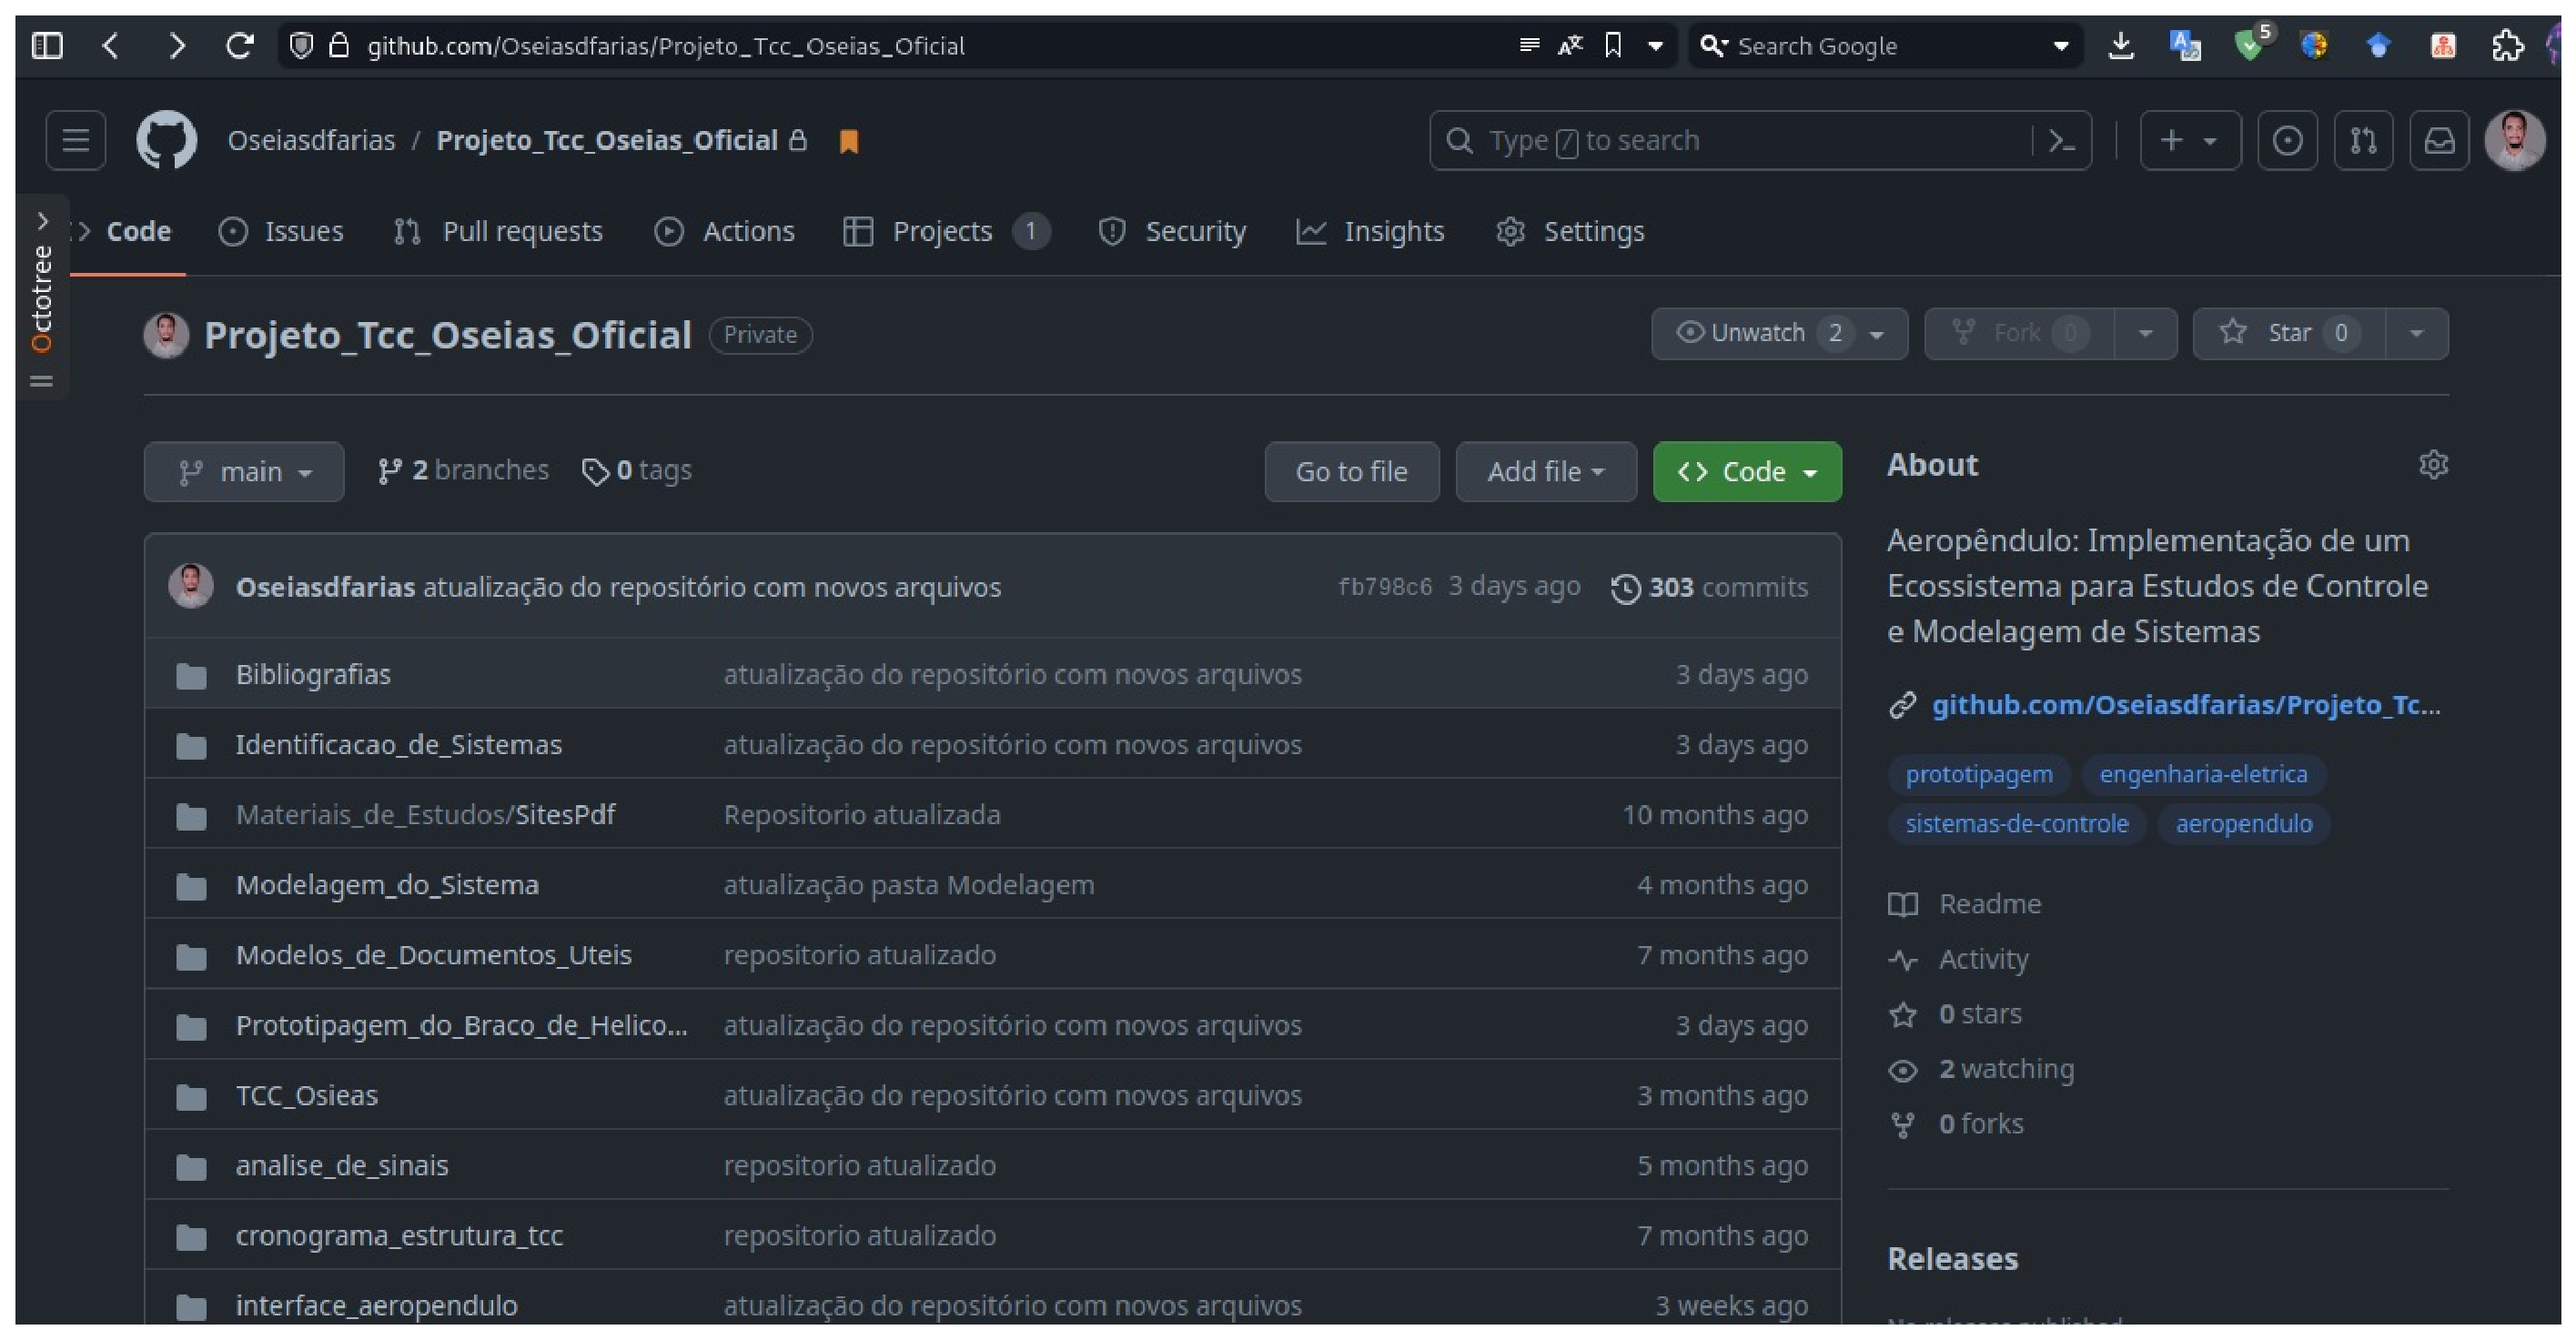
\includegraphics[width=1.0\textwidth]{utils/repo_github.eps}
	\caption*{Fonte: elaborado pelo autor (2023).}
	\label{fig3:image_27}
\end{figure}


% Novo apêndice----------------------------------------------------------------
%\chapter{Nome do outro apêndice}
%\label{chap:apendiceB}
%
%conteúdo do novo apêndice

\end{apendicesenv}
							% Apêndices
	\include{pos-textuais/anexos}								% Anexos
	
\end{document}
